\label{ch:cmanager}

In the previous chapters, we discussed the requirements and support of data-intensive workloads and workflows on high performance computing (HPC) resources.

Executing, though, scientific computational campaigns asks for a software system that provides capabilities to plan and execute multiple workflows on multiple HPC resources.


Currently, there are software systems which support computational campaigns, such as PanDA~\cite{maeno2008panda}, DIRAC~\cite{casajus2010dirac}, QCFractal~\cite{qcfractal}, glideinWMS~\cite{sfiligoi2008glidein}, and others.
PanDA WMS~\cite{maeno2008panda}, is built to support the ATLAS experiment~\cite{atlas} at LHC, and is able to execute several thousand jobs concurrently processing million of tasks per week~\cite{de2015future}.
DIRAC~\cite{tsaregorodtsev2003dirac} is LHCb Monte Carlo production system at CERN.
QCFractal~\cite{qcfractal} is a campaign manager to execute upon large scale quantum chemistry data.
GlideInWMS~\cite{sfiligoi2008glidein} is a more general purpose campaign manager as it was designed to support different use cases.
These are domain specific campaign managers and make assumptions about the underlying software stack, and the type of workflows to be executed.

The existing campaign managers also support a plethora of computing resources, including Grid resources, HPCs and Cloud.
PanDA~\cite{maeno2008panda}, glideinWMS~\cite{sfiligoi2008glidein}, and DIRAC~\cite{casajus2010dirac} mainly support grid resources.
PanDA has been extended to support HPC resources~\cite{de2015future, de2016accelerating}, and clouds~\cite{de2016accelerating}, while glideinWMS~\cite{sfiligoi2008glidein} supports clouds.
QCFractal~\cite{qcfractal} supports a set of heterogeneous resources including local campus clusters, HPC resources and clouds.
In addition, there are workflow management systems on HPCs, like Pegasus~\cite{deelman2015pegasus}, and Balsam~\cite{salim2019balsam}, that support the execution of multiple workflows on HPC resources, but not specifically campaigns.

Existing campaign managers are making assumptions about the resources and middleware they are utilizing.
In addition, they are monolithic software systems, despite their modular design, and tend to be domain specific.
For example, PanDA~\cite{maeno2008panda}, Pegasus~\cite{deelman2015pegasus}, and glideinWMS~\cite{sfiligoi2008glidein} are not easily extensible to use other capabilities or runtime systems.
QCFractal is built to be extensible and be able to interface with different workflow and workload management systems. Currently, it supports multiple execution engines.
As a consequence, domain scientists and user either build custom tools to support their needs or fit their campaigns to a selected software system.


In response to these limitations --- monolithic designs, domain specific support and resource and middleware assumptions --- we designed and prototyped a new campaign manager (CM).
The campaign manager prototype supports use cases from different domains, such as molecular dynamics and earth sciences.
As a result, it is domain agnostic.
In addition, our campaign manager is design by following the building blocks approach~\cite{turilli2019middleware}.
In this way, it will be agnostic of the system used to manage the execution of the campaign workflows.
This, in turn, will allow our CM to make no assumptions about the resources on which the campaign workflows will be mapped and executed.

In this chapter, we discuss the campaign manager requirements as they are derived by the use cases that it supports.
We describe the building blocks approach, the design architecture and implementation of the campaign manager and how it aligns with the building blocks.
Finally, we characterize the overheads of the campaign manager.

\section{Campaign manager requirements}
The requirements for designing a campaign manager can be vast.
We use two real use cases to derive the requirements of the campaign manager prototype.
The first use case supports quantum chemistry campaigns and the second earth sciences.

The quantum chemistry use case (UC1) has O(1k) workflows to execute, and up to 1000 to be executing at any given point in time, to a number of different resources. 
The workflows execution time varies between half-core hours up to 100-core hours.
In addition, users have access to resources with several capabilities and not every workflow can be executed in any resources. 

During the campaign definition, the users may provide an initial workflow priority.
This priority may change during runtime, as users want specific workflows to execute before others.
Furthermore, users may want to early bind workflows to resources, as some resources may already support the required software for a workflow, or have the necessary data there.

The set of resources the user has access to and their availability may change during the lifetime of a campaign.
User may get access to new resources as the campaign is executing, and would like to utilize them for the campaign.
In addition, a resource may become permanently unavailable as the user may lose access while the campaign executes.
The campaign may change during runtime as users add or remove workflows.

The earth science use case (UC2) requires the execution of multiple workflows to analyze images from different calendar years.
Workflows are a set of pipelines over an acquired dataset.
Workflow execution time varies from hours to a couple of days.
Workflows are added to the campaign as data are becoming available.
In addition, due to the data volume this use case requires a shared filesystem between the used resources.

A summary of the functional requirements is shown in Table~\ref{tab:fun_reqs}.

\begin{table}[t]
    \centering
    \scriptsize
    \begin{tabular}{@{}p{1.5cm}|p{2.8cm}p{1.5cm}p{6cm}@{}}
        \toprule
        \textbf{REQ ID} &\textbf{Requirement Algorithm} &\textbf{Use Case} & \textbf{Description} \\
        \midrule
         1 & 
         Support campaign with O(1k) workflows & 
         UC1 & 
         The campaign manager should be able to support campaigns with order of thousand workflows.
         Planning, execution and adaptation should be able to execute with such a campaign.\\
         2 & 
         The CM should support at least two different planning algorithms. & 
         G & 
         Users/developers should be able to easily extend the planning capabilities with algorithms.\\
         3 & 
         Support from 1 up to 100 resources & 
         UC1-UC2 & 
         The CM should be able to execute workflows on multiple resources concurrently.
         These resources can either be actual or emulated resources.\\
         4 & 
         Plan should be derived for heterogeneous and homogeneous static resources in 5 minutes & 
         G & 
         The plan should be derived as soon as the user provides a campaign description. 
         Plan should be derived in less than 5 minutes.\\
         5 & 
         Plan should be derived and adapted for heterogeneous/homogeneous dynamic resources in 5 minutes & 
         UC1 & 
         The plan should be derived as soon as the user provides a campaign description.
         Plan should be derived in less than 5 minutes.
         In case the plan needs to be adapted, it should be adapted in less than 5 minutes.\\
         6 & 
         Interface with different WMFs & 
         G & 
         The campaign manager should be able to interface with different WMFs based on the specifics of the campaign. \\
         7 & 
         Early bind workflows to resources &
         UC1 &
         The user may need to bind workflows to specific resources before executing the campaign.\\
         8 & 
         Campaign objective is configurable & 
         UC1 & 
         While the campaign is executing, the objective may be adjusted based on user preferences.\\
         9 &
         Update the campaign during runtime &
         UC1-UC2 &
         The user may want to update the campaign while it is executing to add/remove workflows.\\
         10 &
         Resources may be added or removed during runtime & 
         UC1 & 
         The user may want to add/remove resources, she has gained/lost access to.\\
        \bottomrule
    \end{tabular}
    \caption{Campaign manager functional requirements.\label{tab:fun_reqs}}
\end{table}

\section{Campaign Manager Design}
This section discusses the design principles and the architecture of the campaign manager.
The design principles the campaign manager follows are presented in ~\S~\ref{ssec:building_blocks}.
The architecture and API of the campaign manager is described in \S~\ref{ssec:cm_arch}.
\subsection{Building Blocks Design Approach}
\label{ssec:building_blocks}
The building blocks approach, as descirbed in~\cite{turilli2019middleware}, defines four design principles for software systems.
Those are self-sufficiency, interoperability, composability, and extensibility.
Adhering to those principles during the design and implementation phase of a software system allows for greater software sustainability.
In addition, it allows users to not tailor their solutions to a specific software ecosystem and take full advantage of the plethora of software that supports scientific computing.

Self-sufficiency and interoperability describe the characteristics of software entities and functionalities.
The entities are enough to stand alone and can be reduced to a specific abstraction.
The functionalities of each building block are specific to the block and do not overlap with other blocks.
As a result, the campaign manager design defines a set of components and that allow it to execute a campaign to HPC resources without providing capabilities to execute the individual workflows of the campaign or acquire the necessary resources.

Composability and extensibility describe the communication and coordination between building blocks and the generality of the generality of the blocks components respectively.
Blocks communicate information about their state, events and errors.
Based on this information alone building blocks are coordinating with each other.
As a result, the campaign manager uses only the state of the workflow execution to create the campaign state.
Furthermore, its components are designed to be general enough so that they can extended and interface with different workflow execution engines as well as software systems that execute computational campaigns.

\subsection{Campaign Manager Components}
\label{ssec:cm_arch}

Figure~\ref{fig:refarch} shows a reference architecture where the CM has three components:
\begin{inparaenum}[(1)]
    \item a Planner;
    \item an Enactor; and
    \item a Bookkeeper. 
\end{inparaenum}
Workflow execution will be managed by an existing workflow management framework (WMF) on HPC resources.
Plan updates will be based on workflows execution metrics provided by the selected WMF such as tasks execution time, overheads calculation and time to completion.
These metrics will be aggregated across workflows, resulting in campaign-wide execution metrics.

\begin{figure*}[t]
    \centering
    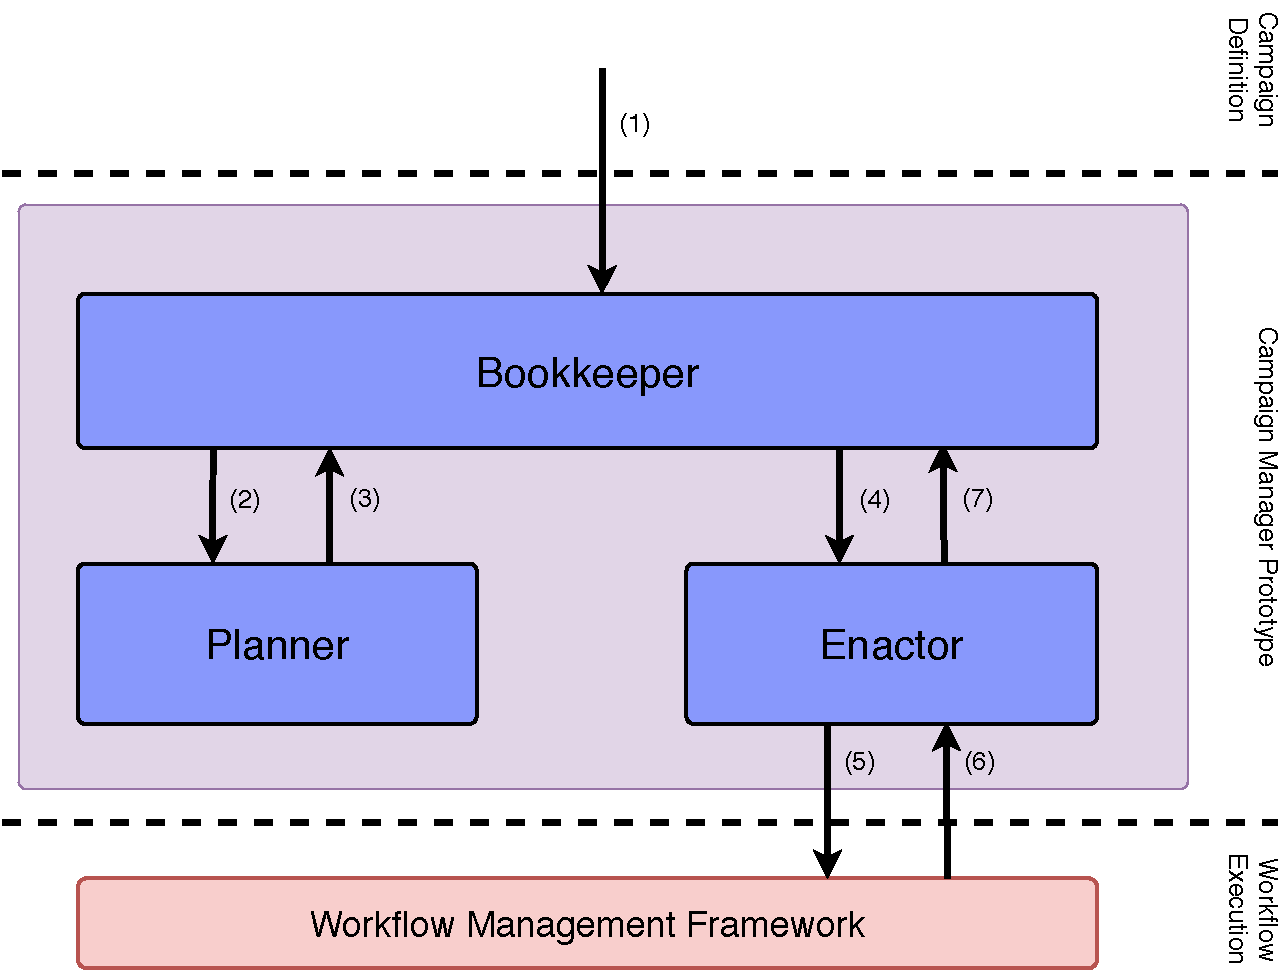
\includegraphics[width=.95\textwidth]{figures/manager/CEM_design.pdf}
    \caption{Reference Architecture of a Campaign Manager. Basic 
        components of Campaign Manager (CM): 1) Planner, 2) Enactor and 3) Bookkeeper. 
        CM communicates decisions to Workflows Management Framework. CM communicates with HPCs to 
        execute parts of the campaign.}\label{fig:refarch}
\end{figure*}

The planner derives an execution plan based on a planning algorithm, calculates the makespan of a campaign based on the set of available resources and the given objective. 
The planner receives information about the state of resources as well as the state of the workflows of the campaign from the bookkeeper component.
In addition, based on information from the other components, the planner might be able to update the plan during the campaign runtime. 

The Bookkeeper component is responsible for monitoring the execution of the campaign.
This component knows the state of the campaign, the execution plan, the availability of the resources, and the campaign's objective.
The state of the campaign will be based on information that the bookkeeper receives from the enactor component.
In addition, the bookkeeper knows the state of the resources the campaign is utilizing at runtime and the state of the resources that are planned to be used.
Based on this set of information, the bookkeeper checks whether the campaign's objective can be achieved.
The bookkeeper will inform the planner to update the plan when changes in the campaign happens that affect the effectiveness of a current plan or make the stated objective not achievable. 
For example, workflows could be removed or added to the campaign, or the availability of one or more resources could change requiring a revision of the mapping of workflows to resources or making such mapping impossible.

The enactor is responsible to execute the planner's plan by interfacing with the WMF.
Based on the plan, the enactor is responsible to execute workflows on the assigned resources.
To achieve that, the enactor informs the WMF to acquire resources, translates the workflow from the user's specification to the API provided by the WMF, and submits the workflow for execution.
Furthermore, the enactor informs the bookkeeper about which workflows were submitted for execution and their state.
%In the case where a group of workflows is to be executed as a single workflow, the enactor will be responsible to group them as well.

\section{Implementation and Overhead Evaluation}
\label{sec:cm_impl}

The campaign manager prototype in accordance with its design defines three major classes.
A bookkeeper class implements the capabilities of the bookkeeper component.
An enactor class interacts with a selected workflow engine to execute worklflows on resources.
A planner class that implements planning algorithms.
In addition, it defines a state model for the campaign and the workflows.

The states models provide information about the state of the execution.
The campaign state model has four states: 1) new, 2) planning, 3) executing and 3) final.
A campaign is considered \textit{new} when it is defined and no further action is taken.
It goes to state \textit{planning} when a plan for its execution is derived.
As soon as the execution of the campaign starts, the state transitions to \textit{executing}.
The final state is a set of possible termination states.
When the campaign execution ends and the campaign objective is achieved, the state transitions to \textit{done}.
If the objective cannot be achieved or there is a failure during the execution, the state changes to \textit{failed}.
Lastly, the campaign state goes to \textit{canceled} when the user cancels the execution of the campaign.


Figures~\ref{fig:rcm_class_diagram} and~\ref{fig:seq_diagram} show the class diagram of the prototype and the sequence diagram of executing a campaign.
We define three classes based on each component of the reference architecture.
Each class also defines a set of data structures to support the execution.

\begin{figure*}[t]
    \centering
    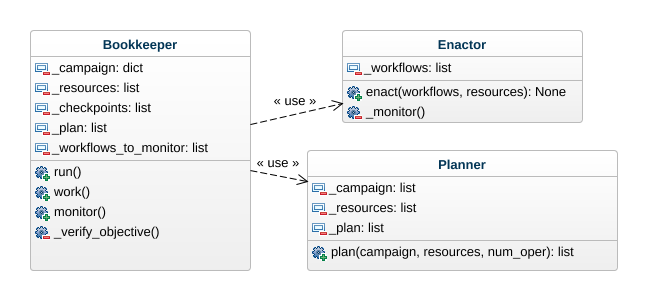
\includegraphics[width=.95\textwidth]{figures/manager/class_diagram.png}
    \caption{Class diagram of campaign manager prototype}\label{fig:rcm_class_diagram}
\end{figure*}

The Bookkeeper class defines the necessary methods and parameters to execute a campaign.
The most important methods are \textit{run}, \textit{work} and \textit{monitor}.
Method \textit{run} initializes the campaign state to \textit{new} and sets up the environment for executing the campaign.
\textit{Work} calls the planner to produce a plan transitioning the state of the campaign to \textit{planning}.
After a plan is produced, \textit{work} via calling \textit{\_verify\_objective} checks if the objective of the campaign can be achieved and starts submitting workflows to the enactor.
In addition, it pushes the submitted workflows to a data structure that the \textit{monitor} method reads.
The \textit{monitor} method checks the state of the workflow execution as given by the enactor.



\begin{figure*}[t]
    \centering
    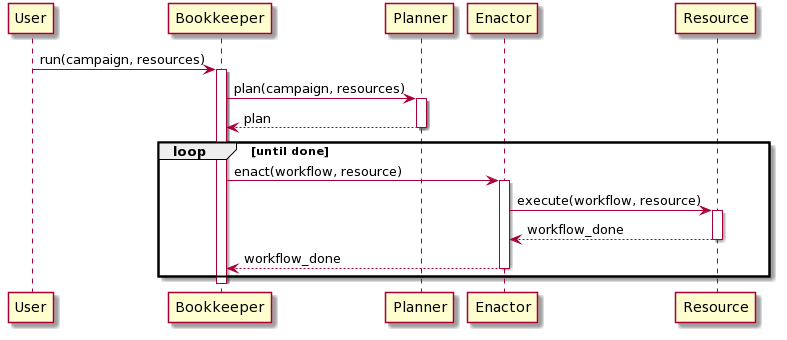
\includegraphics[width=.95\textwidth]{figures/manager/rcm_seq.png}
    \caption{Basic sequence diagram of executing a campaign via the campaign manager}\label{fig:seq_diagram}
\end{figure*}



